\documentclass[12pt,a4paper]{article}
\usepackage[utf8]{inputenc}
\usepackage{amsmath}
\usepackage{textcomp}

\usepackage{geometry}
\geometry{a4paper,left=25mm,right=25mm, top=2cm, bottom=2cm} 

\usepackage{verbatim}

 \usepackage{mathptmx}
 \usepackage[scaled=.90]{helvet}
 \usepackage{courier}

\usepackage[utf8]{inputenc}

\usepackage{listings}
\usepackage{color}

\usepackage{graphicx}
 
\definecolor{dkgreen}{rgb}{0,0.6,0}
\definecolor{gray}{rgb}{0.5,0.5,0.5}
\definecolor{mauve}{rgb}{0.58,0,0.82}

\pagestyle{empty}
\lstset{numbers=left,language=C++}
\lstset{showstringspaces=false,
basicstyle=\ttfamily\footnotesize,
breaklines=true,
tabsize=3,
commentstyle=\color{dkgreen},       % comment style
}

%keine einrückungen bei absatz
\parindent 0pt

\begin{document}
\title{Übung 4}
\author{Bernhard Selymes, Reinhard Penn}
\date{November 2012}

\normalsize

%Pfad zu c++ Dateien
\newcommand{\CodePath}{../ImageManagment/ImageManagment/}

%Beginn des Dokuments
\section{Organisatorisches}

\subsection{Team}
	\begin {itemize} 
		\item Reinhard Penn, s1110306019 
		\item Bernhard Selymes, s1110306024
	\end {itemize}

\subsection{Aufteilung}
	\begin {itemize} 
		\item Reinhard Penn
			\begin {itemize}
				\item Planung
				\item Klassendiagramm
				\item Implementierung der Klassen SingletonBase, ImageManagement, Circle, EmptyGraphicObjectFactory
				\item Testen aller Klassen
			\end {itemize}
		\item Bernhard Selymes
			\begin {itemize}
				\item Planung
				\item Klassendiagramm
				\item Implementierung der Klassen Image, Rectangle, FilledGraphicObjectFactory, GraphicObject
				\item Dokumentation			
			\end {itemize}
	\end {itemize}


\subsection{Zeitaufwand}
	\begin {itemize}
		\item geschätzte Mh: 20h
		\item tatsächlich: Reinhard (10h), Bernhard  (9h)
	\end {itemize}


\section{Systemspezifikation}

Es soll für die beiden Firmen Epcos und Nortel Networks ein Verschlüsselungssystem mit jeweils einem firmeneigenen Interface entworfen werden. Die geforderte Verschlüsselungssoftware soll in der Lage sein Daten mithilfe des Caesar und RSA Algorithmus zu verschlüsseln und entschlüsseln.
\newline
Das Interface der Firma Epcos bietet nur die RSA Verschlüsselung an.
\newline
Das Interface der Firma Nortel Networks bietet beide Verschlüsselungsalgorithmen an. Der entsprechende Algorithmus wird mithilfe einer Enumeration ausgewählt.
\\


\newpage
\section {Systementwurf}

\subsection {Klassendiagramm}

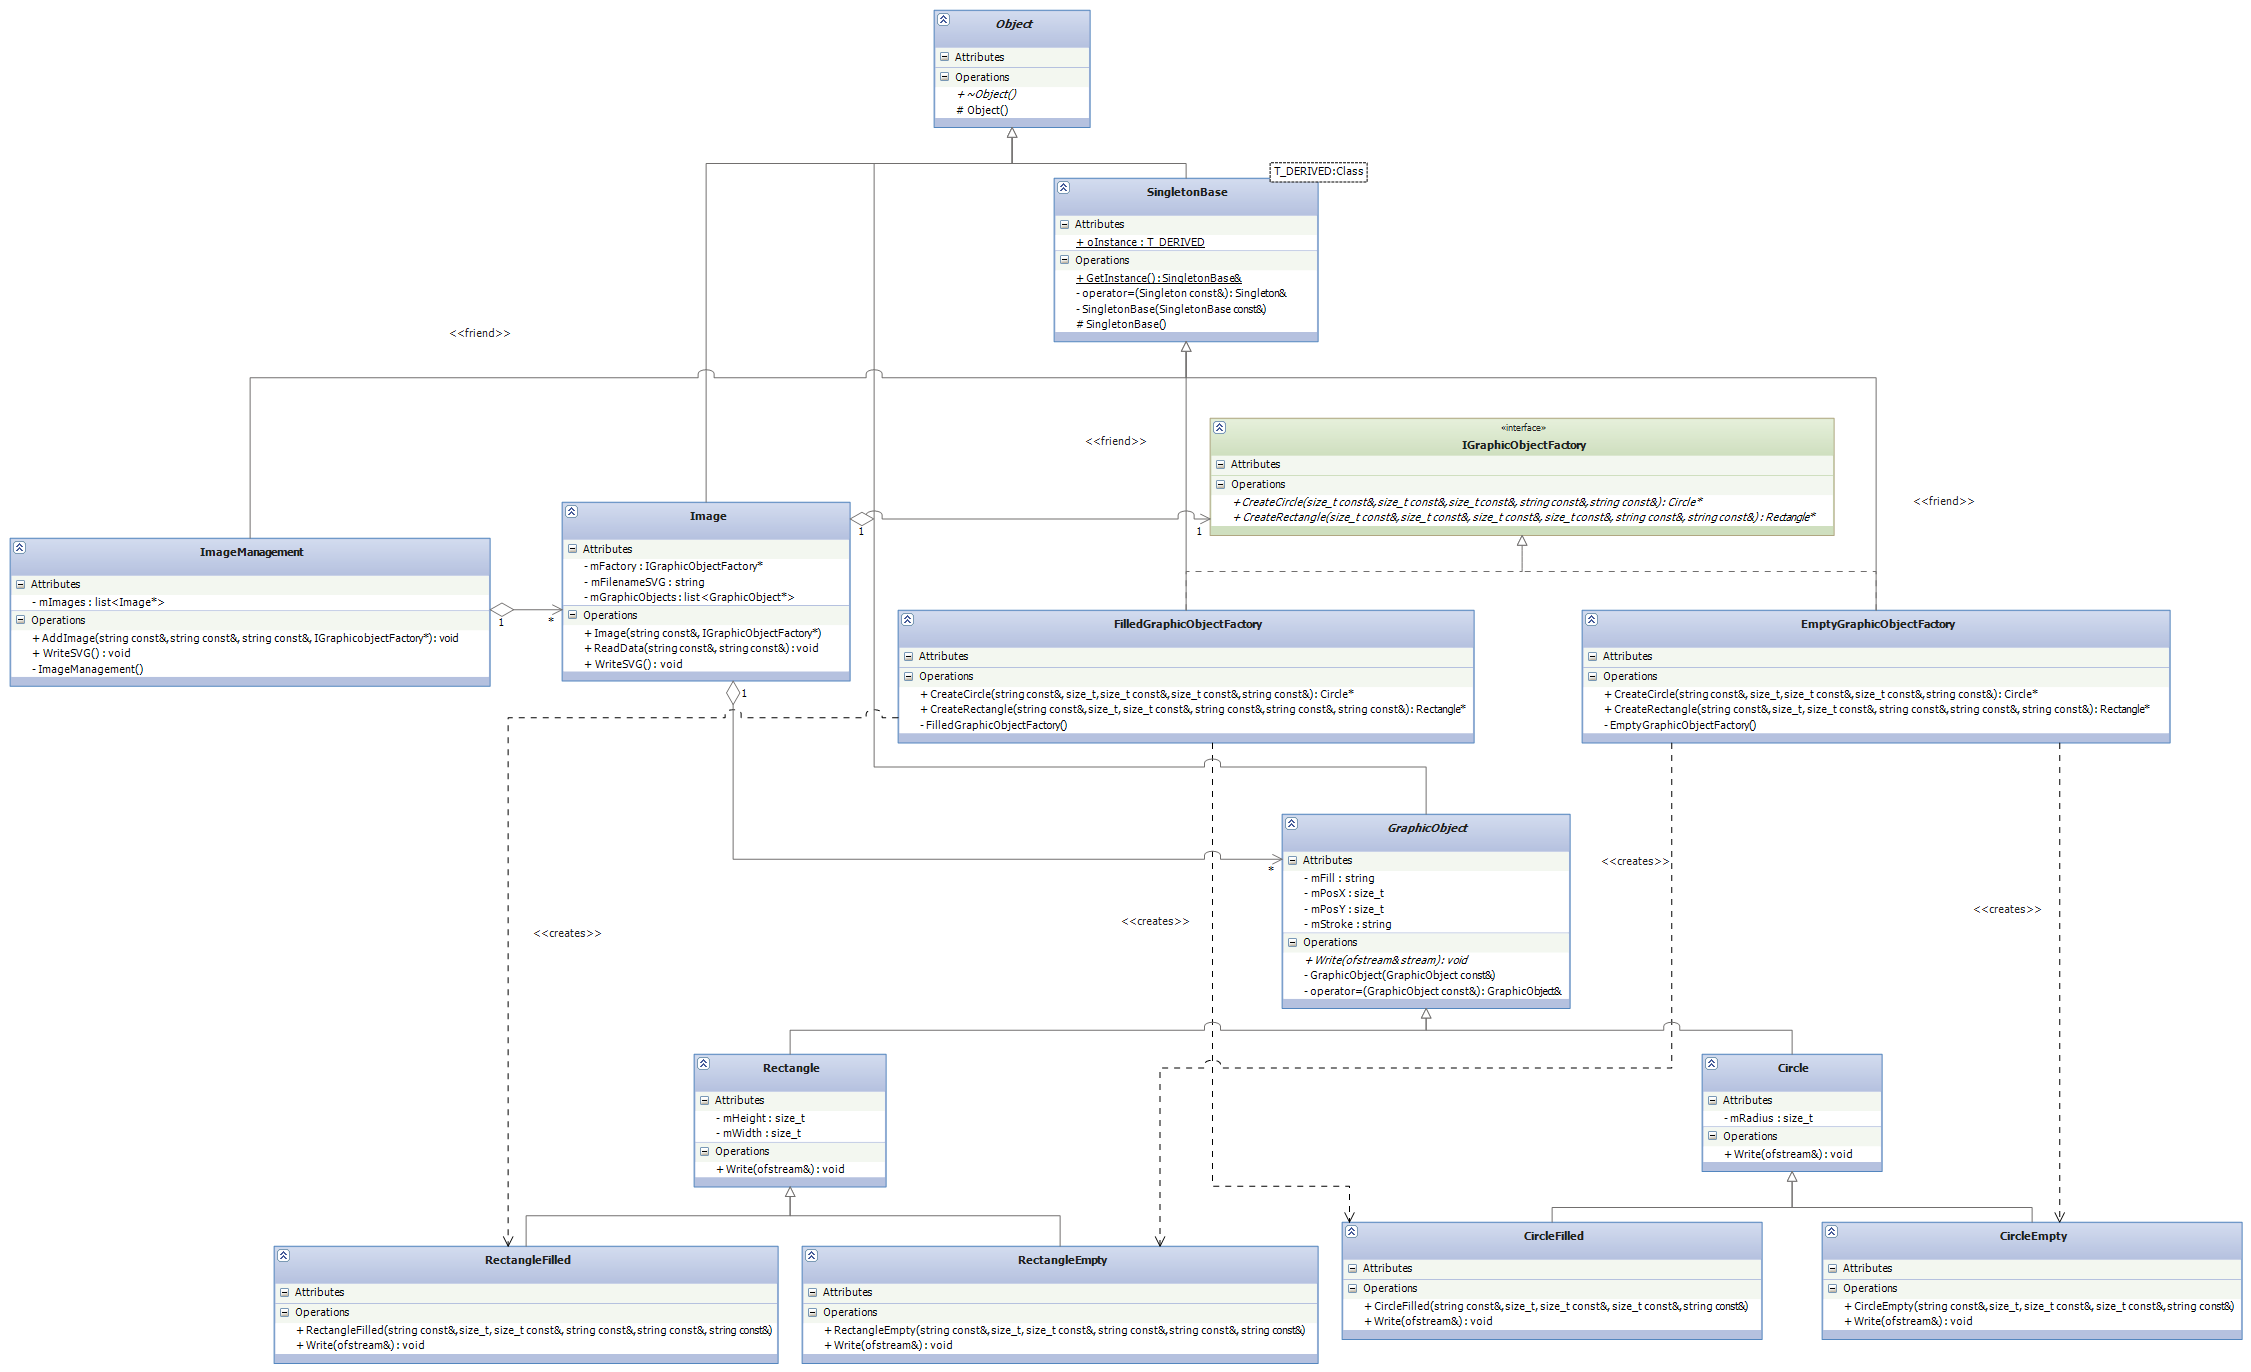
\includegraphics[angle=90,scale=0.6] {../Klassendiagramm.png}

\newpage
\subsection {Komponentenübersicht}
\begin {itemize} 
	\item Klasse "Object":
	\newline
	Basis aller Basisklassen.
	
	\item Klasse "Cryptographer":
	\newline
	Basisklasse für der Verschlüsselungsalgorithmen.
	
	\item Klasse "CryptographerCaesar":
	\newline
	Stellt den Caesar Algorithmus bereit.
	
	\item Klasse "CryptographerRSA":
	\newline	
	Stellt den RSA Algorithmus bereit.
	
	\item Interface "IEpcos":
	\newline
	Interface für die Firma Epcos. Stellt nur RSA zur Verfügung.
	
	\item Interface "INortelNetworks":
	\newline
	Interface für die Firma NortelNetworks. Stellt RSA und Caesar zur Verfügung.
	
	\item Klasse "EpcosAdapter":
	\newline
	Implementiert das Interface "IEpcos".
	
	\item Klasse "NortelNetworksAdapter":
	\newline
	Implementiert das Interface "INortelNetworks".
	
	\item Enumeration "TEncoding":
	\newline
	Dient zur Auswahl des Verschlüsselungsalgorithmus.
	
	
\end {itemize}

\newpage
\section {Komponentenentwurf}
\subsection {Klasse "Object"}
Abstrakte Basisklasse aller Klassen. Von ihr werden alle anderen Klassen abgeleitet. Beinhaltet einen virtuellen Destruktor.


\subsection {Klasse "Cryptographer"}
Hat einen String in dem der aktuelle Fileinhalt gespeichert wird.
\\

\textbf {Methode "Decrypt": } 
\newline
Schnittstelle: 
Rückgabetyp: void.
\newline
Pure virtual function.
\\

\textbf {Methode "Encrypt": } 
\newline
Schnittstelle:
\newline
Rückgabetyp: void.
\newline
Pure virtual function.
\\

\textbf {Methode "ReadFile": } 
\newline
Schnittstelle:
\newline
Parameter: string const\& filename.
\newline
Rückgabetyp: void.
\newline
Liest ein File mithilfe von FileToString ein.
\\

\textbf {Methode "WriteFile": } 
\newline
Schnittstelle: 
\newline
Parameter: string const\& filename.
\newline
Rückgabetyp: void.
\newline
Schreibt die Daten in mData in ein File.
\\

\textbf {Methode "FileToString": } 
\newline
Schnittstelle: 
\newline
Parameter: string const\& filename.
\newline
Rückgabetyp: void.
\newline
Schreibt die Daten der Datei in den member mData.
\\


\subsection {Klasse "CryptographerCaesar"}
Ermöglicht es Daten mithilfe des Caesar Algorithmus zu verschlüsseln und entschlüsseln.
\\

\textbf {Methode "Decrypt": } 
\newline
Schnittstelle: 
Rückgabetyp: void.
\newline
Ruft für jeden Character von mData die Funktion DecryptCaesar auf.
\\

\textbf {Methode "Encrypt": } 
\newline
Schnittstelle:
\newline
Rückgabetyp: void.
\newline
Ruft für jeden Character von mData die Funktion EncryptCaesar auf.
\\

\textbf {Methode "EncryptCaesar": } 
\newline
Schnittstelle: 
\newline
Parameter: char\& ch.
\newline
Rückgabetyp: void.
\newline
Verschlüsselt den aktuellen character.
\\

\textbf {Methode "DecryptCaesar": } 
\newline
Schnittstelle: 
\newline
Parameter: char\& ch.
\newline
Rückgabetyp: void.
\newline
Entschlüsselt den aktuellen character.
\\


\subsection {Klasse "CryptographerRSA"}
Ermöglicht es Daten mithilfe des RSA Algorithmus zu verschlüsseln und entschlüsseln.
\\

\textbf {Methode "Decrypt": } 
\newline
Schnittstelle: 
Rückgabetyp: void.
\newline
Ruft für jeden Character von mData die Funktion DecryptRSA auf.
\\

\textbf {Methode "Encrypt": } 
\newline
Schnittstelle:
\newline
Rückgabetyp: void.
\newline
Ruft für jeden Character von mData die Funktion EncryptRSA auf.
\\

\textbf {Methode "EncryptRSA": } 
\newline
Schnittstelle: 
\newline
Parameter: char\& ch.
\newline
Rückgabetyp: void.
\newline
Ruft für jeden character die Funktion PowerModulo mit den entsprechenden Werten auf.
\\

\textbf {Methode "DecryptRSA": } 
\newline
Schnittstelle: 
\newline
Parameter: char\& ch.
\newline
Rückgabetyp: void.
\newline
Ruft für jeden character die Funktion PowerModulo mit den entsprechenden Werten auf.
\\

\textbf {Methode "PowerModulo": } 
\newline
Schnittstelle: 
\newline
Parameter: int x, int ed.
\newline
Rückgabetyp: void.
\newline
Berechnet folgenden Ausdruck: x\^(e|d) mod n.
\\


\subsection {Klasse "INortelNetworks"}
Bietet jeweils eine Funktion zum ent- und verschlüsseln an. Der Algorithmus wird mithilfe einer Enum festgelegt.
\\

\textbf {Methode "Decipher": } 
\newline
Schnittstelle:
Parameter: TEncoding encoding, std::string const\& filename
Rückgabetyp: void.
\newline
Pure virtual function.
\\

\textbf {Methode "Encipher": } 
\newline
Schnittstelle:
Parameter: TEncoding encoding, std::string const\& filename
Rückgabetyp: void.
\newline
Pure virtual function.
\\


\subsection {Klasse "NortelNetworksAdapter"}
Implementiert das Interface INortelNetworks. Je nach Verschlüsselungsart wird ein dynamischer Cryptographer angelegt, entweder vom Typ RSA oder Caesar. Nach dem De-/Encipher Aufruf wird dieser wieder freigegeben.
\\

\textbf {Methode "Decipher": } 
\newline
Schnittstelle:
Parameter: TEncoding encoding, std::string const\& filename
Rückgabetyp: void.
\newline
Die Datei wird mithilfe des entsprechenden Cryptographers ausgelesen und entschlüsselt. Danach wird mit ihm eine neue unverschlüsselete Datei erstellt. Die Dateiendung wird auf .txt gesetzt.
\\

\textbf {Methode "Encipher": } 
\newline
Schnittstelle:
Parameter: TEncoding encoding, std::string const\& filename
Rückgabetyp: void.
\newline
Die Datei wird mithilfe des entsprechenden Cryptographers ausgelesen und verschlüsselt. Danach wird mit ihm eine neue verschlüsselte Datei erstellt. Die Dateiendung entspricht dabei der jeweiligen Verschlüsselungstechnick.
\\


\subsection {Klasse "IEpcos"}
Bietet jeweils eine Funktion zum ent- und verschlüsseln an. Der Algorithmus ist nicht wählbar, es wird immer RSA verwendet.
\\

\textbf {Methode "DecryptRSA": } 
\newline
Schnittstelle:
Parameter: std::string const\& filename
Rückgabetyp: void.
\newline
Pure virtual function.
\\

\textbf {Methode "EncryptRSA": } 
\newline
Schnittstelle:
Parameter: std::string const\& filename
Rückgabetyp: void.
\newline
Pure virtual function.
\\


\subsection {Klasse "EpcosAdapter"}
Bietet jeweils eine Funktion zum ent- und verschlüsseln an. Der Algorithmus ist nicht wählbar, es wird immer RSA verwendet. Die Ver-/Entschlüsselung erfolgt durch einen dynamisch angelegten CryptographerRSA.
\\

\textbf {Methode "DecryptRSA": } 
\newline
Schnittstelle:
Parameter: std::string const\& filename
Rückgabetyp: void.
\newline
Die Datei wird mithilfe des CryptographerRSA ausgelesen und entschlüsselt. Danach wird mit ihm eine neue entschlüsselte Datei erstellt. Die Dateiendung wird auf .txt gesetzt.
\\

\textbf {Methode "EncryptRSA": } 
\newline
Schnittstelle:
Parameter: std::string const\& filename
Rückgabetyp: void.
\newline
Die Datei wird mithilfe des CryptographerRSA ausgelesen und verschlüsselt. Danach wird mit ihm eine neue verschlüsselte Datei erstellt. Die Dateiendung wird auf .RSA gesetzt.
\\



\newpage
\section {Source Code}

\lstinputlisting[language=C++]{\CodePath Object.h}
\lstinputlisting[language=C++]{\CodePath Object.cpp}
\newpage

\lstinputlisting[language=C++]{\CodePath Cryptographer.h}
\newpage
\lstinputlisting[language=C++]{\CodePath Cryptographer.cpp}
\newpage

\lstinputlisting[language=C++]{\CodePath CryptographerCaeser.h}
\newpage
\lstinputlisting[language=C++]{\CodePath CryptographerCaeser.cpp}
\newpage

\lstinputlisting[language=C++]{\CodePath CryptographerRSA.h}
\newpage
\lstinputlisting[language=C++]{\CodePath CryptographerRSA.cpp}
\newpage

\lstinputlisting[language=C++]{\CodePath INortelNetworks.h}
\lstinputlisting[language=C++]{\CodePath NortelNetworksAdapter.h}
\newpage
\lstinputlisting[language=C++]{\CodePath NortelNetworksAdapter.cpp}
\newpage

\lstinputlisting[language=C++]{\CodePath IEpcos.h}
\lstinputlisting[language=C++]{\CodePath EpcosAdapter.h}
\newpage
\lstinputlisting[language=C++]{\CodePath EpcosAdapter.cpp}
\newpage

\section {Testausgaben} 

\begin {verbatim}
Visual Leak Detector Version 2.2.3 installed.
Testcase0: File doesnt exist
Encrypt with Epcos, RSA: testcase0.txt ...
EpcosAdapter::EncryptRSA: File couldn't be opened
Finished
Decrypt with Epcos, RSA: testcase0.txt.RSA ... 
EpcosAdapter.cpp::DecryptRSA: File couldn't be opened
Finished
Encipher with NortelNetworks, RSA: testcase0.txt ... 
NortelNetworksAdapter::Encipher: File couldn't be opened
Finished
Decipher with NortelNetworks, RSA: testcase0.txt.RSA ... 
NortelNetworksAdapter::Decipher: File couldn't be opened
Finished
Encipher with NortelNetworks, Caesar: testcase0.txt ... 
NortelNetworksAdapter::Encipher: File couldn't be opened
Finished
Decipher with NortelNetworks, Caesar: testcase0.txt.Caesar ...
NortelNetworksAdapter::Decipher: File couldn't be opened
Finished
Testcase1: File is empty
Encrypt with Epcos, RSA: testcase1.txt ... Finished
Decrypt with Epcos, RSA: testcase1.txt.RSA ... Finished
Encipher with NortelNetworks, RSA: testcase1.txt ... Finished
Decipher with NortelNetworks, RSA: testcase1.txt.RSA ... Finished
Encipher with NortelNetworks, Caesar: testcase1.txt ... Finished
Decipher with NortelNetworks, Caesar: testcase1.txt.Caesar ... Finished
Testcase2: Ascii symbols
Encrypt with Epcos, RSA: testcase2.txt ... Finished
Decrypt with Epcos, RSA: testcase2.txt.RSA ... Finished
Encipher with NortelNetworks, RSA: testcase2.txt ... Finished
Decipher with NortelNetworks, RSA: testcase2.txt.RSA ... Finished
Encipher with NortelNetworks, Caesar: testcase2.txt ... Finished
Decipher with NortelNetworks, Caesar: testcase2.txt.Caesar ... Finished
Testcase3: Normal text
Encrypt with Epcos, RSA: testcase3.txt ... Finished
Decrypt with Epcos, RSA: testcase3.txt.RSA ... Finished
Encipher with NortelNetworks, RSA: testcase3.txt ... Finished
Decipher with NortelNetworks, RSA: testcase3.txt.RSA ... Finished
Encipher with NortelNetworks, Caesar: testcase3.txt ... Finished
Decipher with NortelNetworks, Caesar: testcase3.txt.Caesar ... Finished
No memory leaks detected.
Visual Leak Detector is now exiting.
Drücken Sie eine beliebige Taste . . .
\end {verbatim}


\end{document}